
% Prepared by Calvin Kent
%
% Assignment Template v19.02
%
%%% 20xx0x/MATHxxx/Crowdmark/Ax
%
\documentclass[12pt]{article} %
\usepackage{amsthm}
\usepackage{CKpreamble}
\usepackage{CKassignment}
\usepackage{mdframed}
\usepackage{import}
\usepackage{pdfpages}
\usepackage{transparent}
\usepackage{xcolor}
\usepackage{tkz-euclide}
\usepackage{physunits}
\usepackage{physics}
\usepackage{lmodern}
\usepackage{microtype}
\usepackage{upgreek}
\usepackage[misc]{ifsym}

%%% Maths and science packages

\usepackage{amsmath,amsthm,amssymb}
\usepackage{pgfplots}
	\usetikzlibrary{
		calc,
		patterns,
		positioning
	}
	\pgfplotsset{
		compat=1.16,
		samples=200,
		clip=false,
		my axis style/.style={
			axis x line=middle,
			axis y line=middle,
			legend pos=outer north east,
			axis line style={
				->,
			},
			legend style={
				font=\footnotesize
			},
			label style={
				font=\footnotesize
			},
			tick label style={
				font=\footnotesize
			},
			xlabel style={
				at={
					(ticklabel* cs:1)
				},
				anchor=west,
				font=\footnotesize,
			},
			ylabel style={
				at={
					(ticklabel* cs:1)
				},
				anchor=west,
				font=\footnotesize,
			},
			xlabel= $x$,
			ylabel=$\vec d (\m \tx{[East]})$
		},
	}
	\tikzset{
		>=stealth
	}

%%% Tables and figures packages

\usepackage{float}
\usepackage{caption}
	\captionsetup{
		format=plain,
		labelfont=bf,
		font=small,
		justification=centering
	}
	


\theoremstyle{ex}
\newtheorem*{ex}{Example}

\newcommand{\incfig}[2][1]{%
    \def\svgwidth{#1\columnwidth}
    \import{./figures/}{#2.pdf_tex}
}

\pdfsuppresswarningpagegroup=1

\newcounter{step}[section]
\newenvironment{step}[1][]
{\refstepcounter{step} \textbf{Step #1.}}


%
\begin{document}
	\pagenumbering{arabic}
	% Start of class settings ...
	\renewcommand*{\coursecode}{MATH 235} % renew course code
	\renewcommand*{\assgnnumber}{Assignment 1} % renew assignment number
	\renewcommand*{\submdate}{September 14, 2021} % renew the date
	\renewcommand*{\studentfname}{Abdullah} % Student first name
	\renewcommand*{\studentlname}{Zubair} % Student last name
    \renewcommand*{\proofname}{Proof:}
	% \renewcommand*{\studentnum}{20836288} % Student number

	\renewcommand\qedsymbol{$\blacksquare$}
	\setfigpath
	% End of class settings	
	% \pagestyle{crowdmark}
	\newgeometry{left=18mm, right=18mm, top=22mm, bottom=22mm} % page is set to default values
	\fancyhfoffset[L,O]{0pt} % header orientation fixed
	% End of class settings
	%%% Note to user:
	% CTRL + F <CHANGE ME:> (without the angular brackets) in CKpreamble to specify graphics paths accordingly.
	% The command \circled[]{} accepts one optional and one mandatory argument.
	% Optional argument is for the size of the circle and mandatory argument is for its contents.
	% \circled{A} produces circled A, with size drawn for letter A. \circled[TT]{A} produces circled A with size drawn for TT.
	% https://github.com/CalvinKent/My-LaTeX
	%%%

	%%%%%%%%%%%%%%%%%%%%%%%%%%%%%%%%%%%%%%%%%%%%%%%%%%%%%%%%%%%%%%%%%%%%%%%%%%%%%%%
	%%%                        CUSTOM MACRO VIM-TEX                             %%%
	%%       call IMAP('NOM', '\nomenclature{}', 'tex')               

	%%%%%%%%%%%%%%%%%%%%%%%%%%%%%%%%%%%%%%%%%%%%%%%%%%%%%%%%%%%%%%%%%%%%%%%%%%%%%%%

	% Crowdmark assignment start
	% qnumber, qname, qpoints

\begin{center}
		\Huge{\underline{\textbf{How to go from Factored to Vertex form}}}
\end{center}

\begin{ex}
  We first cover a few examples of quadratics in factored form. \textbf{(IN class)}
\end{ex}
We are trying to convert from factored form to vertex form,
\[
   f(x) = b(mx \pm t)(nx \pm s)  \longrightarrow f(x) = a(x - h)^2 + k
.\] 
\begin{step}[1]
  Set both factors equal to $0$, and solve,
  \begin{align*}
    factor_1 & = 0\\
    factor_2 &= 0
  .\end{align*}
  After you have your x-intercepts, label them $x_1$ and $x_2$. (The order of assignment doesn't matter)
\end{step}

\begin{step}[2]
  Calculate $h$ by,
  \[
        h = \frac{x_1 + x_2}{2}
  .\] 
\end{step}

\begin{step}[3]
  Calculate $k$ by,
  \[
        k = f(h)
  .\] 
\end{step}

\begin{step}[4]
  Calculate $a$ by,
  \[
        a = b\cdot m\cdot n
  .\] 
\end{step}


\begin{step}[5]
  Write down the equation in vertex form,
   \[
        f(x) = a(x-h)^2 + k
  .\] 
\end{step}


\textbf{\underline{\Large{Practice Problems:}}}
\begin{qstn}
  Convert the following quadratics to vertex form.
  \begin{enumerate}[label=(\alph*)]
    \item $g(x) = -4(x - 4)(x-6)$
    \item $A(x) = -x(4x+16)$
    \item $f(x) = (7 - x)(3 - x)$
    \item $\kappa(x) = (-2x+14)(x-5)$
    \item $\mu(x) = -(x+8)(8x+24)$
    \item $T(x) = (3x+6)(-2x-8)$
    \item $\eta(x) = (6x-12)^2$
  \end{enumerate}
\end{qstn}

\begin{qstn}
  A quadratic function has x-intercepts $x_1 = 5, x_2 = -1$. It also has the point $(1,8)$. Determine the equation of the
  quadratic function in vertex form, and also provide a sketch of the function. \textbf{Label:} The \emph{y-intercept},\,\, \emph{the
    vertex}, and the \emph{x-intercepts}.
  \[
      f(x) = a(x-h)^2 + k
  .\] 
\end{qstn}

\newpage
\textbf{\underline{\Large{Solutions to Practice Problems:}}}\\
\textbf{Question 1.} Solution:
 \begin{enumerate}[label=(\alph*)]
   \item $g(x) = -4(x-5)^2 + 4$
   \item $A(x) = -4(x+2)^2 + 16$
   \item $f(x) = -(x-5)^2 + 4$
   \item $\kappa(x) = -2(x-6)^2 + 2$
   \item $\mu(x) = -8\left(x+\frac{11}{2}\right)^2 + 50$
   \item $T(x) = -6(x+3)^2 + 6$
   \item $\eta(x) = 36(x-2)^2$
 \end{enumerate}


\textbf{Question 2.} Solution:
\[
      f(x) = -(x-2)^2 + 9
.\] 
    \begin{center}
        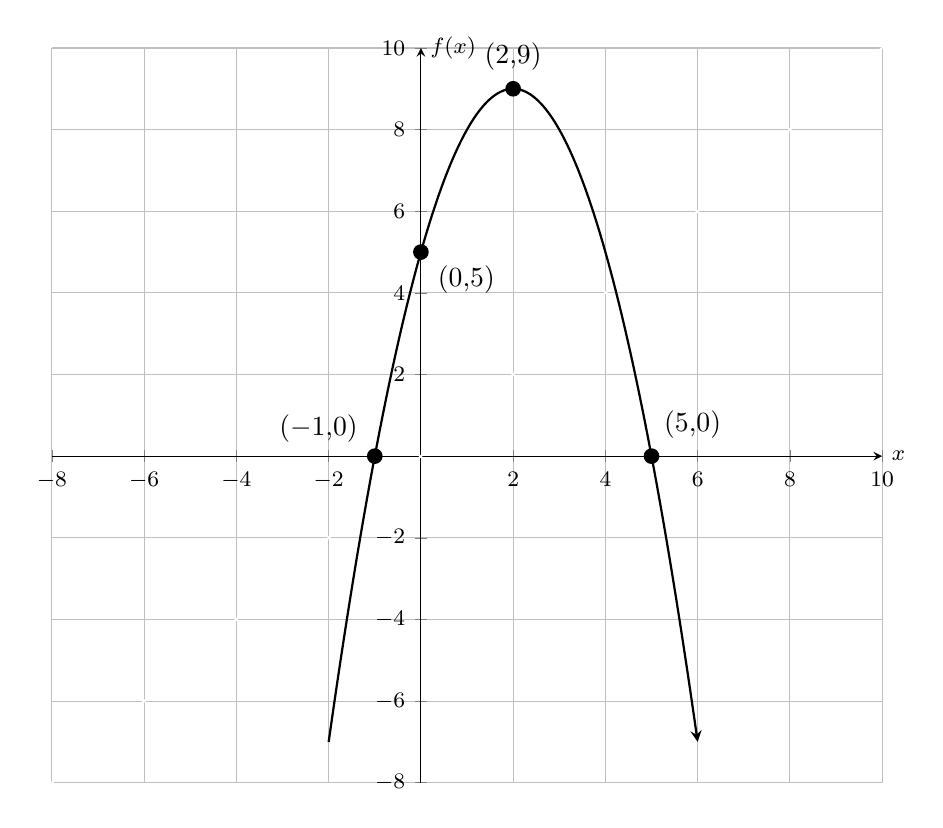
\begin{tikzpicture}
        \begin{axis}[
            my axis style,
            width=\textwidth,
            height=0.9\textwidth,
            ylabel=$f(x)$,
            grid
        ]
        
        \addplot[
            domain=-8:10,
            thick,
            white,
            -
        ]
        {x};

        \addplot[
            domain=-2:6,
            thick,
            black,
            ->
        ]
        {-(x-2)^2+9};

        \fill[
            black
        ];


        \node[label={90:{($2$,$9$)}},circle,fill,inner sep=2pt] at (axis cs:2,9) {};
        \node[label={330:{($0$,$5$)}},circle,fill,inner sep=2pt] at (axis cs:0,5) {};
        \node[label={70:{($5$,$0$)}},circle,fill,inner sep=2pt] at (axis cs:5,0) {};
        \node[label={150:{($-1$,$0$)}},circle,fill,inner sep=2pt] at (axis cs:-1,0) {};
     

        \end{axis}
        \end{tikzpicture}
    \end{center}


\end{document}





